\section{Background}
{\color{red}---Catchy first sentence.}\newline
\textit{Machine learning} aims to infer generally valid relationships from a finite set of training data and apply those learned relations to new data \cite{domingos2012few} \cite{kotsiantis2007supervised}. While some problems can be solved by manually encoding explicit rules, others require a different approach as explicit decision-making does not deliver highly accurate results \cite{burrell2016machine}. Determining a student's grade in a multiple choice test can be solved by explicitly encoding mathematical rules, yet deciding whether the tonality of a text is positive or negative needs more than a simple rule set to function accurately \cite{melville2009sentiment}. The datasets needed to train machine learning models are often large and represented in a high-dimensional feature space, which makes it impossible for a human to carry out the learning task like a machine can. However, machines can be used to extend the cognitive capabilities of humans when working together on those learning tasks. \cite{ventocilla2018taxonomy} describes the fruitful collaboration between human and machine as \textit{augmented intelligence}, pointing at the positive aspect of machine learning support.\newline
{\color{red}---Narrowing topic to decision-making and discriminative algorithms and define "decision" as output from ML systems}


%------------------------------------------------------------------
\subsection{Interpretability in AI}
Humans cooperating with machines need to understand the principles of the method that is employed - a property referred to as \textit{transparency} \cite{kotsiantis2007supervised}. \textit{Opacity}, the direct opposite of transparency \cite{lipton2016mythos}, is a major problem for augmented intelligence. Although opacity can be used voluntarily as a means to self-protection and censorship, it also arises involuntarily due to missing technical expertise and failed human intuition and cognitive abilities \cite{burrell2016machine}.\newline
On the application-side of machine learning systems, the question of transparency brings up the notion of \textit{interpretability}. Interpretability refers to how well a ``typical classifier generated by a learning algorithm" can be understood \cite{kotsiantis2007supervised}, as compared to the theoretical principle of the method. That is, an interpretable machine learning system is either inherently interpretable, meaning that its operations and result patterns can be understood by a human \cite{biran2017explanation} \cite{ventocilla2018taxonomy}, or it is capable of generating descriptions understandable to humans \cite{gilpin2018explaining}. It is also possible to equip a system retrospectively with interpretability by adding a proxy model capable of mirroring the original system's behaviour while being comprehensible for humans \cite{guidotti2018survey}. Using an interpretable system as a human means being enabled to make inferences about underlying data \cite{ventocilla2018taxonomy}.\newline
\cite{guidotti2018survey} assigns ten desired dimensions to interpretable machine learning systems:
\begin{itemize}
	\item \textit{Scope}: Global interpretability (understanding the model and operations) and local interpretability (understanding what brought about a single decision)
	\item \textit{Timing}: Time scope available in the application use case for a target user to understand 
	\item \textit{Prior knowledge}: Level of expertise of target user
	\item \textit{Dimensionality}: Size of the model and the data
	\item \textit{Accuracy}: Target accuracy of the system while maintaining interpretability
	\item \textit{Fidelity}: Accuracy of explanation vs. accuracy of model
	\item \textit{Fairness}: Robustness against automated discrimination and ethically challenging biases in data
	\item \textit{Privacy}: Protection of sensible and personal data
	\item \textit{Monotonicity}: Level of monotonicity in relations of input and output (human intuition is largely monotonic)
	\item \textit{Usability}: Efficiency, effectiveness, and joy of use
\end{itemize}
In the context of interpretability for machine learning systems, the terms \textit{understandability}, \textit{comprehensibility}, \textit{explainability}, and \textit{justification} are often mentioned in literature. In this paper, we adopt the definition of \cite{ruping2006learning}. \textit{Understandability}, \textit{accuracy} of the explanation, and \textit{efficiency} of the explanation together form \textit{interpretability}. \textit{Explainability} is a synonym of \textit{comprehensibility} \cite{weihs2003combining}, which is also synonymic to \textit{understandability} \cite{bibal2016interpretability} and therefore an aspect of interpretability, showing the reasons for the system's behaviour \cite{gilpin2018explaining}. Figure \ref{fig:definitions} gives an overview over these terms. Finally, \textit{justification} refers to the evidence for why a decision is correct, which does not necessarily include the underlying reasons and causes \cite{biran2017explanation}.\newline
\begin{figure} [h]
	\centering
	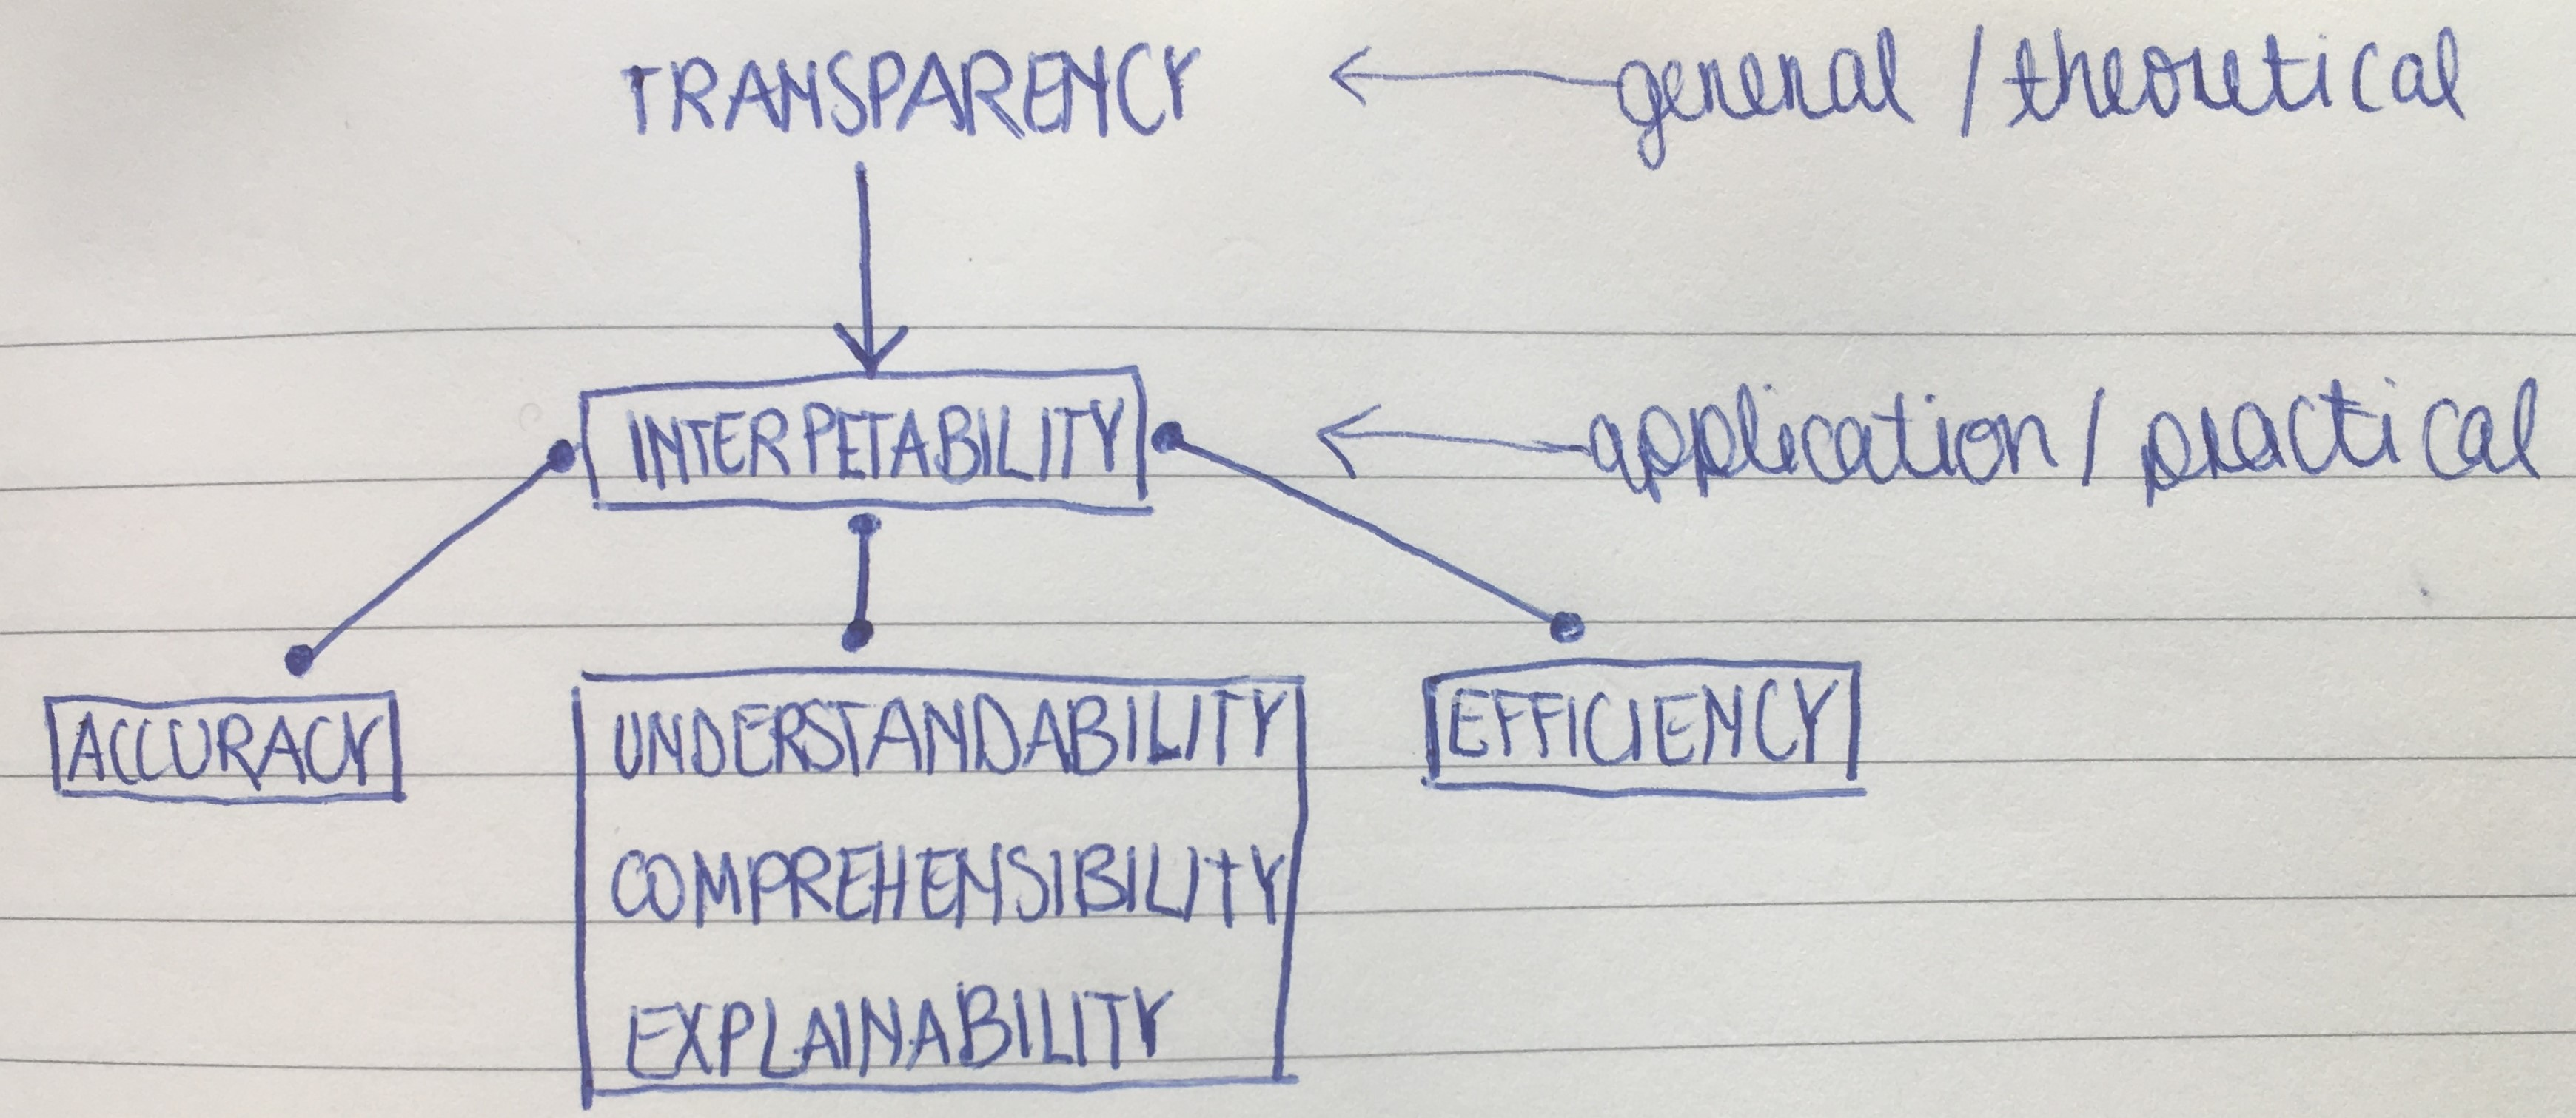
\includegraphics[width=0.7\linewidth]{img/definitions}
	\caption{Relation of terms connected to interpretability}
	\label{fig:definitions}
\end{figure}
If the human cognition is augmented by a machine learning system, talking about interpretability should also include discussing the interpretability of the human in the loop. \cite{lipton2016mythos} argues that human behaviour is often mistakenly identified as interpretable, since humans can explain their actions and beliefs. However, the actual operations of the human brain remain opaque, which refutes interpretability \cite{lipton2016mythos}. Human interpretability is not the focus of this paper and will therefore not be discussed in the remainder, yet it should serve as a point of reference for the general discussion of algorithmic interpretability.\newline





%------------------------------------------------------------------
\subsection{Need for Explainability in AI}
A subfield of artificial intelligence research revolves solely around the explainability of intelligent systems: \textit{xAI}, explainable artificial intelligence, for the purpose of enabling communication with agents about their reasoning \cite{hendricks2018generating}. xAI systems face a trade-off challenge: Their explanation has to be complete and interpretable at the same time \cite{gilpin2018explaining}. The attention span an cognitive abilities of humans therefore become an important factor to consider in the design of a xAI systemm \cite{kulesza2013too}. Furthermore, the goal of explaining the system is twofold: create actual knowledge and persuade the user that the knowledge is sound and complete. Actual understanding and perceived understanding however do not always go hand in hand: Persuasive systems can convince the user without creating actual transparency \cite{gilpin2018explaining}. Bad explanations likewise ``provide an understanding that is at best incomplete and at worst false reassurance" \cite{burrell2016machine}. Next to examining possible explanations for white box (inherently interpretable) and black box (inherently non-interpretable) systems, the design and communication of explanations need to be considered as well. \cite{guidotti2018survey}\newline
In recent years, machine learning algorithms employed in the wild show a trend towards increasing accuracy but also increasing complexity. In general, the higher the accuracy and complexity, the lower the explainability \cite{richardson2018survey} \cite{chen2018learning} in machine learning. However, users do not necessarily perceive systems with simple explanations as more understandable \cite{allahyari2011user}. The authors of the user study in \cite{allahyari2011user} hypothesise that users detect missing information in simple explanations, which in turn leads to the perception of incomprehensibility. \cite{van2018contrastive} examined user preferences in more detail and concluded that users overall preferred more soundness and completeness over simplicity, as well as global explanations over local explanations.\newline
Humans involved in the explanation process are not only users, but also domain experts and engineers during the design and training phase. As explanations are user-dependent (not monolithic) \cite{preece2018asking}, the design and evaluation of explanation needs to be conducted in reference to the target users. Including experts in the modelling and training process is not only a way to integrate expert knowledge that is otherwise difficult to model, but can also increase user trust \cite{ventocilla2018taxonomy}. \cite{liu2017towards} call the situation where a human expert works alongside the machine learning system to improve it ``mixed initiative guidance". \newline

\paragraph{Goals of Explainability}
To achive transparency and accountability [14] \newline
Right for the right reasons: not enough to just be correct, the reasons need to be correct. Example of things going wrong without noticing: [56] \newline
for users: trust, for engineers: debugging and improving [14]\newline
trust when it comes to critical decisions (e.g. medical diagnosis) [29] \newline

user-related goals: \newline
Scrutability, trust, effectiveness, efficiency, satisfaction, persuasiveness [2] \newline
Explainability improves the user's confidence in the system, user's trust, user's judgement ability on prediction correctness, user satisfaction, user acceptance [10] \newline
acceptance, trust, perceived competence [59] \newline
acceptance, appropriate trust [38] \newline

\paragraph{Issues with Opacity}
\begin{itemize}
	\item high cost of errors in high-risk domains [2] [8] [17]
	\item human safety in safety-critical tasks [6] [15]
	\item automated discrimination [2], biased training data [6] [15] [24]
	\item censorship [2]
	\item development: fine-tuning parameters with trial-and-error [4]
	\item imperceptibly altered input data or altered model: criminals / hackers [6]
	\item unintuitive systematic errors [6] [56] [24]
	\item regulations: right to explanation [1] [6] [8]
	\item source of knowledge that should be accessible if needed [8] [15]
	\item (inappropriate) trust into the system (either too much or too little) [15] [14] [17] [24]
	\item implementation involves a lot of human work [33]
\end{itemize}
need dependent on consequences of classification results [15]:
\begin{itemize}
	\item \textbf{no need} for interpretability if no consequences arise from faulty decisions
	\item interpretability is \textbf{beneficial} if consequences for individuals arise from faulty decisions
	\item interpretability is \textbf{critical} if serious consequences arise from faulty decisions
\end{itemize}
need also dependent on user role [38] \newline

\paragraph{Barriers to Interpretability}
intentional concealment, lack of technical expertise, computational complexity vs. human-scale reasoning abilities [1] \newline
minimum explainability: how features (values) relate to predictions [1] \newline

\paragraph{Regulations}
General Data Prodection Regulation (GDPR): law about processing of personal (related to identifiable person) data, no matter if manually or automatically processed [1] \newline
Sensitive data / protected traits: race, ethnicity, religion, nationality, gender, sexuality, disability, marital status, age [2] \newline
Real-life data contains society's structures and biases, and as classification means separation into groups based on that data, biases are taken into the model [1] \newline
\begin{itemize}
	\item minimal interpretation: delete sensitive data from dataset
	\item maximum interpretation: delete sensitive data and correlated variables from dataset
\end{itemize}
``right to explanation" [1], argument against such interpretation [58] and positive interpretation [37]. Key issue: ``data subjects receive meaningful, but properly limited, information" [58] is ambiguous, plus no clear definition of explanation, meaningful, and information. Summary: Precedents are needed to clarify the boundaries.\newline
Problem with explanations: ML algorithms show statistical correlation, not causality [1]\newline


\paragraph{Accountability}
information worth disclosing for more accountability [2]:
\begin{itemize}
	\item human involvement: who controls the algorithm, who designed it etc., leading to control through social pressure
	\item data statistics (accuracy, completeness, uncertainty, representativeness), labelling \& collection process, preprocessing of data
	\item model: input, weights, parameters, hidden information
	\item inferencing: covariance matrix to estimate risk, prevention measures for known errors, confidence score 
	\item algorithmic presence: visibility, filtering, reach of algorithm
\end{itemize}

\paragraph{Persuasiveness}
persuasiveness of explanation != actual explanation [10]\newline
``High-fidelity explanations, also referred to as faithful, have a strong correspondence between the explanation model and the underlying machine learning model" [51]\newline
``[Persuasive explanations] are less faithful to the underlying model than descriptive explanations in a tradeoff for more freedom on the explanation complexity, structure, and parameters. This freedom permits explanations better tailored to human cognitive function, making them more functionally interpretable." [51]\newline
``Descriptive explanations best satisfy the ethical goal of transparency" [51]\newline






%------------------------------------------------------------------
\subsection{Application Areas}

\subsubsection{Application Areas}
decisions that affect people’s lives in critical domains like criminal
justice, fair lending, and medicine. [52]\newline
safety-critical industries (self-driving cars, robotic assistants, personalised medicine) [3]\newline

sensitive data processed by algorithms (banks, insurances, health data) [3]\newline

scientific research (making discoveries by understanding data) [3]\newline

individual performance monitoring, health care, economic situation analysis, personal preferences \& interests, location \& movement [1]\newline

replacing human decision making in advertising, recommendations, finances (loans) [6] \newline

health care, recommender systems, planning, HRI [15]\newline

medicine, finances, criminal justice [19] \newline

education, health care, manufacturing, retail, when machine learning based support systems are used [16] \newline

high-risk domains: medical diagnosis, terrorism detection [24] \newline

``socially consequential mechanisms of classification and ranking" [33] \newline

spam detection, finances (fraud detection, loan), search engines, news trends, marketing, insurance [33] [36] \newline

\subsubsection{Exemplary Failures}
examples of failures due to missing explanation:
[3]:
\begin{itemize}
	\item St Georges hospital - racist application procedure 
	\item COMPASS crime prediction - racist against blacks (counterargument made in [55]: ``group differences in scores may reflect true differences in recidivism risk")
	\item Amazon prime district selection - defavorising neighborhoods with ethnic minorities
	\item Automated target identification - decision driven by weather condition
	\item Animal race 
	\item Mortgage rates of major US banks rate very differently - sign for bad algorithms?
\end{itemize}
``Discrimination, is at some level, inherent to profiling: the point of profiling is to treat some people differently" [57]:
\begin{itemize}
	\item Discrimination of women: ads of higher-paid jobs more often shown to men than to women (but no reason given, may be intentional)
\end{itemize}
[54]
\begin{itemize}
	\item researcher group is the main reason for variance, not classifier etc., hence human bias in ML
\end{itemize}
[14]
\begin{itemize}
	\item Google Flue Trends: systematic modelling error 
\end{itemize}







%------------------------------------------------------------------
\subsection{Explanations}
Explanation = reasons or justification for an action or belief [14]\newline

Function of explanations:\newline
\begin{itemize}
	\item prediction of consequences of (similar) events in the future [11] [5]
	\item control of events  [5]
	\item building and refining inner knowledge model [5]
	\item restauration / prevention of states or events [11]
	\item comparison of methods [11]
	\item reproduction of states or events [11]
	\item assigning guilt [11] [5]
	\item justification [11] [5]
	\item persuasion [5]
	\item pleasure / appreciation [11]
\end{itemize}

\subsubsection{Human-Human Explanations}
explanations are not mental model but rather the interpretation of relations [11]\newline
explanations are less general than theories and are application-focussed [11] \newline
explanations are a cognitive and social process: The challenge of explaining includes finding a complete but compressed explanation, and transferring the explanation from the explainer to the explainee [5].\newline
Complete explanation == all relevant causes explained [5] \newline

Explanation aspects [11]:
\begin{itemize}
	\item causal pattern content: common-cause, common-effect, linear chain, homeostatics
	\item explanatory stance types: mechanical, design, intention stance [5]. Atypical stances can lead to distorted understanding.
	\item explanatory domain: different fields have different preferences of explanation types
	\item social-emotional content: can alter acceptance threshold and influence recipient's perception of explained event 
\end{itemize}
What constitutes a \textbf{good explanation}? [11] describes good explanations as being non-circular, showing coherence, and having a high relevance for the recipient. Circularity are causal chains where an effect is given as cause to itself (with zero or more causal steps in between). Explanations can, but do not have to, explain causal relations [11]. Especially in the case of machine learning algorithms, the learned model shows correlation, not causation. Explanations for statistical models therefore cannot draw on typical causal explanations as found in human-human communication {\color{red}[REF NEEDED]}. The probabilistic interpretation of causality comes closest to the patterns learned in statistical models: If an even $A$ caused an event $B$, then the occurrence of $A$ increases the probability of $B$ occurring. Statistical facts are not satisfactory elements of an explanation, unless explaining the event of observing a fact [5]. Arguably, this holds true for statistical learning. Coherence refers to the systemacity of explanation elements: good explanations do not hold contradicting elements, but elements that influence each other [11]. Finally, relevance is driven by the level of detail given in the explanation. The sender has to adapt the explanation to the recipient's prior knowledge level and cognitive ability to understand the explanation [5], which can mean to generalise and to omit information - [11] calls this adaptation process the ``common informational grounding". The act of explaining also includes a broader grounding of shared beliefs and meanings of events and the world [5]. The ``compression problem" poses a major challenge in constructing explanations for humans. Humans tend to not comprise all possible causes and aspects of the high-dimensional real world in an explanation, suggesting that there are compression strategies (on the sender's side) and coping strategies (on the recipient's side) in place [11]. \newline
[5] notes that besides presenting likely causes, and coherence, a good explanation is simple and general. The latter two characteristics refer to the agreement widely accepted in science that a simple theory (or, in this case, an explanation) is favoured over a more complicated theory if both explain an equal set of events or states.\newline
[21] defines a good explanation as sound, complete, but nor overwhelming. While soundness refers to the level of truthfulness, completeness describes the level of disclosure [21]. In order to avoid overwhelming the explainee, the informational grounding process takes place, i.e. a common understanding of related elements and an adaptation of the explanation's detailedness to the explainee's knowledge level.\newline

Generally, the more diverse the given evidence, the higher the recipient's \textbf{acceptance} of the explanation [11].\newline

Cultural differences exist for the preference of an explanation type, although all explanation types can be understood [11].\newline

Humans build \textbf{mental models} of the world, a mental representation of events or elements. Mental models are needed to explain and predict. We do not need to have complete, holistic mental models in order to use an artifact, but a ``functional" model is needed to tell us how to use and make use of it, while a ``structural" model stores information about the composition and how it is built [21]. \newline

mindlessness and explanations [32]\newline

\paragraph{Explanation Types}
associations between antecedent and consequent, contrast and differences, causal mechanisms [10] \newline
material cause, formal / categorical cause, efficient cause, final cause [5] \newline


\subsubsection{AI-Human Explanations}
Focus:\newline
[10]:
\begin{itemize}
	\item feature-level: feature influence, intersection of actual \& expected contribution per feature
	\item sample-level: explanation vector, linguistic explanation for textual data using BOW, subtext as justification for class (trained independently), caption generation 
	\item model-level: rule extraction, prototypes \& criticism samples representing model, proxy model (inherently interpretable) with comparable accuracy (NOTE: supposedly meant decision generation, not simple accuracy)
\end{itemize}
single focus: feature-based explanation best for recommender systems (as compared to similar previous decisions and similar neighbor decisions) [10] \newline
[4]:
\begin{itemize}
	\item understanding and reassurance (right for the right reasons)
	\item diagnosis (of errors, inacceptable performance or behaviour)
	\item refinement (improving robustness and performance)
\end{itemize}
[6]:
\begin{itemize}
	\item representation of data \& features
	\item processing of data (operations)
	\item explanation generation (within model)
\end{itemize}
[5]:
\begin{itemize}
	\item computational / operations level
	\item representational level
	\item hardware level
\end{itemize}
[8]:
\begin{itemize}
	\item learning algorithm behaviour
	\item model parameters
	\item model itself
	\item representation
\end{itemize}
[15]:
\begin{itemize}
	\item within algorithm, directly based on model
	\item feature-based
	\item secondary, add-on explanation system separate from learning algorithm
	\item representation
\end{itemize}
[14]:
\begin{itemize}
	\item inner workings for transparency
	\item post-hoc prediction visualisation, e.g. heat maps
\end{itemize}
[16]:
\begin{itemize}
	\item dataset / features
	\item optimizer / learning algorithm
	\item model 
	\item prediction / result
	\item evaluator
\end{itemize}

\textbf{Explanation selection}: it is not possible to show every case, parameter, feature importance to the user, therefore a selection of exemplary cases needs to be made [24]. Global explanation can originate from a set of representative cases [24].



\subsubsection{When to explain?}
[15] stresses that different explainability needs call for different timings of the explanation. Showing the explanation \textbf{before} a classification or generation task is useful for justifying the next step or explaining the plan. {\color{green}\textbf{During} a task, information about the operations and features can help identifying errors for correction and foster trust.} Explaining the results of a task \textbf{after} the process is useful for reporting and knowledge discovery.



\subsubsection{Explanation Systems}
For models that are not inherently interpretable, the explanation can only be an approximation and cannot be complete (definition of non interpretable) [5]. There can be approximations for the computation / operations detecting properties and categorisations, and approximations of the decision behaviour [5].\newline

counterfactual explanation [12] with fact \& foil \newline
[4] for overview over solutions for understanding, diagnosis, refinement \newline
[6] for overview of solutions for explaining features, operations, generative explanations \newline
[16] for solutions for dataset, optimizer, model, predictor and evaluator \newline
[14] for set of programs (MYCIN, NEOMYCIN, CENTAUR, EES) that try to model explanations alongside with system \newline
[19] presenting the L2X system\newline
[24] Explanation software: LIME, ELUCIDEBUG

For feature-based models, [19] suggests salience map masks on input features, comparable cases (input and output) as reference (or very dissimilar cases as counterfactuals), and mutual information analysis per feature. For the latter, they use the Kullback-Leibler divergence to calculate the mutual information of two vectors: Learning to explain (L2X).\newline

Inherently interpretable / transparent models:
\begin{itemize}
	\item decision trees (graphical representation), rules (textual representation), linear models (feature magnitude and sign) [3]
	\item shallow rule-based models, decision lists, decision trees, feature selection, compositional generative models [10]
	\item decision trees, Naive Bayes, Rule-Learners [71]
\end{itemize}

[{\color{red}REF NEEDED}] add-on and post-hoc systems might be good as explaining, but this fact in itself does not guarantee a sound, i.e. truthful, explanation, ``however plausible they appear" [31]. \newline

[15] suggests to develop a new class of learning algorithms that have an inherent ``explainability hyperparameter" to achieve high accuracy AND high explainability.\newline

[36] argues that most high-dimensional real-world application data is ``concentrated on or near a lower-dimensional manifold" [36], dimension reduction techniques like PCA or other feature selection algorithms can therefore be used to overcome the curse of dimensionality. \newline

\textbf{explanations for texts}:
[7] solution to recent development in text mining, where texts are represented in a high-dimensional vector space (e.g. fasttext, word2vec) and classified with neural nets. Compared to BOW/SVM, the W2V/CCN they used yields equally good results, because the CNN is better at identifying characteristic words.\newline
[19] designed a system that uses deep neural networks for classification and mutual information for getting the input feature importance (in their case, single words). \newline

\textbf{Relevant words}: A word is relevant to the text if removing it from the texts and classifying again results in a decrease of the classification score across all texts







%------------------------------------------------------------------
\subsection{Explanation Evaluation}
[6]:
\begin{itemize}
	\item application grounded: true context, true task, users
	\item human-grounded: usability tests, human performance tests
	\item functionally grounded: no users, proxy
\end{itemize}
[8] evaluation of model interpretability:
\begin{itemize}
	\item heuristics: number of rules, number of nodes, minimum description length (model parameters)
	\item generics: ability to select features, ability to produce class-typical data points, ability to provide information about decision boundaries
	\item specifics: user testing / perception (BUT: evaluation of visuals and perceived model rather than actual model), e.g. by measuring accuracy of prediction, answer time, answer confidence, understanding of model
\end{itemize}
[15] rather combination than only a single one:
\begin{itemize}
	\item algorithm performance score
	\item user performance score
	\item user satisfaction score 
\end{itemize}







%------------------------------------------------------------------
\subsection{Trust in AI}
[25] notes that there exists no precise definition of trust in the field of computer science\newline

[TRUST 02] examined the concept of trust in close relationships and define it as the willingness to put oneself at a risk and believing that the other will be benevolent. They grouped aspects of interpersonal trust into a model with three components: faith, dependability, predictability [TRUST 02]. \newline
Placed in agent, not a characteristic inherent to an agent [TRUST 02]\newline
Trust is a subjective experience rather than objectively measurable [TRUST 05] [23]. \newline
dynamic: evolves as relationship matures [TRUST 02]\newline
attribution of characteristics, e.g. dependability (repeated confirmation in risky situations), reliability (consistency or recurrent behaviour) [TRUST 02]\newline
inappropriate trust can be harmful [17]\newline
Trust as experience, trustworthiness is the characteristic and in case of computer programs consists of factors such as security, privacy, dependability, usability, correctness [TRUST 05] [TRUST 06]. Trust relates to the assurance that a system performs as expected [TRUST 05]. \newline
Trust in a system can be misused: e-crime with negative side effects, e.g. data misuse [TRUST 05]. \newline 

\subsubsection{Gaining User Trust}
Trust factors: appeal, competence (privacy, security, functionality), transparency, duration (relationship, affiliation), reputation [23] \newline
Concerning algorithms, users can put global trust into the system, which means trusting the model itself. Trust can also be assigned locally, into an individual decision. [24] \newline
Trust dimensions of web systems: target (the entity being evaluated), representation (encoding of trust via social warranty, certificates, etc.), method (security), management (the entity putting trust into the system), computation (evaluation metric), purpose [25] \newline
For classification: expectation mismatch leads to direct decrease in trust [30], strength of decrease depends on the type of mismatch. Data-related mismatch weights less strongly than logic-driven mismatch. [30] \newline 
[31] argues that trust in machine learning algorithms also depends on the characteristics of misclassified cases. He points out that an automatic system can be considered trustworthy if it behaves exactly like humans, i.e. it misclassifies the same data points as a human and is correct on those cases that a human would also correctly classify [31].

\subsubsection{Trust Evaluation}
[23]: using experts to assign a weighted label to each element on a website or GUI and calculating a score
\begin{itemize}
	\item [-1] irritant
	\item [1] chaotic
	\item [2] assuring
	\item [3] motivating
	\item [0] not present
\end{itemize}
But user study showed that experts find it problematic to assign discrete trust values. The advantage of this approach, however, is that it is possible to compare multiple websites [23]. \newline
user study with closed and open questions [24]:
\begin{itemize}
	\item Do you trust this algorithm to work well in the real world?
	\item Why do you trust this algorithm to work well in the real world?
	\item How do you think the algorithm distinguished between the two classes?
	\item How certain are you of the correctness of your explanation? 
\end{itemize}
[TRUST 02] develops a trust scale with 26 items, each belonging to one of the three trust factors (faith, dependability, predictability). \newline
[TRUST 01] describes online trust (websites) as developing from external factors (website's reputation, navigational architecture, user's prior experience) as well as perceived factors (credibility, ease of use, risk) \newline
{\color{green}``willingness to accept a computer-generated recommendation is considered a proxy measure of trust" [38] }

\subsubsection{Perceived Understanding}
Perceived understanding important for trust (rather than actual understanding):\newline
``Findings show that the transparent version was perceived as more understandable and perceived understanding correlated with perceived competence, trust and acceptance of the system. Future research is necessary to evaluate the effects of transparency on trust in and acceptance of user-adaptive systems" [59] \newline
Most questionnaires use factual statements to investigate perceived understanding. Participants rate the statements according to their confidence of understanding [UND 03] [UND 07] or directly their subjective understanding [UND 01] [UND 02] [UND 04] [UND 05]



%------------------------------------------------------------------
\subsection{Use Case Scenario}
definition of offensive language [34] \newline
hate speech detection systems \newline








%------------------------------------------------------------------
\subsection{Summary}
Summary\newline
\begin{itemize}
	\item summary scenario
	\item systems
	\item evaluation of explanations and of trust
\end{itemize}
Hypotheses













